\section{Функциональное проектирование}
\label{sec:func}

\subsection{Класс \texttt{QTestPrinter}}
Класс \texttt{QTestPrinter} является реализацией блока тестирования специального принтера.
Данный класс выполняет поиск подключенных принтеров, проверку правильности настроек принтера,
позволяет осуществить проверку состояния принтера путем печати тестовой страницы. Пример тестовой страницы приведен на
рис.\ref{fig:func:sample_page}.
\begin{figure}[!htb]
	\centering
	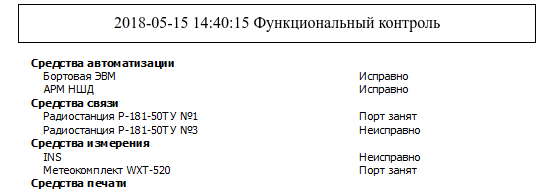
\includegraphics[scale=1.0]{sample_page}
	\caption{Пример тестовой страницы}
	\label{fig:func:sample_page}
\end{figure}

Класс \texttt{QTestPrinter} включает в себя следующие методы:

\begin{enum}
	\item Метод \texttt{test} проводит процедуру тестирования принтера. Данный метод принимает ссылку на строку
		\texttt{sRez}. Данная строка служит для логгирования процесса тестирования устройства. Метод \texttt{test} производит
		проверку наличия принтера и корректности настроек его подключения. В случае, если принтер подключен корректно, создается
		диалоговое окно для печати тестовой страницы. Для формирования тестовой страницы служит метод \texttt{print}, который
		связан с сигналом \texttt{paintRequested}. Сигнал \texttt{paintRequested} посылается при необходимости
		класса Qt \texttt{QPrintPreviewDialog} сгенерировать изображения для предпросмотра печатаемых страниц.

	\item Метод \texttt{print} осуществляет формирование тестовой страницы и выполняет настройку параметров печати. \texttt{print}
		принимает в качестве параметра указатель на класс \texttt{QPrintPreviewDialog}, который используется для настройки
		параметров печати.
\end{enum}

\subsection{Класс \texttt{VTest\_BINS3}}
Данный класс отвечает за тестирование БИНС, работающей по протоколу БИНС-3.

Класс \texttt{VTest\_BINS3} имеет следующие методы и внутренние переменные:
\begin{enum}
	\item Переменная \texttt{m\_bReceiveMess81} является флагом, который выставляется при получении сообщения
		статуса БИНС-3. Сообщение статуса имеет идентификатор 0x81.

	\item Переменная \texttt{m\_bReceiveMess01} - флаг, отвечающий за получения сообщения с навигационными данными.
		Данное Сообщение имеет идентификатор 0x01.

	\item Метод \texttt{onReadFromBins} принимает полученную с БИНС дейтаграмму в виде \texttt{QByteArray}.
		и осуществляет определение типа полученной команды. После определения типа команды устанавливается
		соответствующий флаг.

	\item Метод \texttt{onReadFromSocket} выполняет чтение данных из сокета, через который идет общение с БИНС,
		метод вызывается при появлении информации для чтения с БИНС(сигнал \texttt{readyRead}).
		Данный метод принимает полученную с БИНС дейтаграмму в виде \texttt{QByteArray}.
		При считывании байт команды дейтаграмма передается в метод \texttt{onReadFromBins} для определения типа
		команды.

	\item \texttt{test} является основным методом класса \texttt{VTest\_BINS3}. Данный метод отвечает
		непосредственно за управление тестированием БИНС. Метод проверяет подключение БИНС, настройки и
		параметры подключения устройства. При успешном получении сообщения с навигационными данными и сообщения
		статуса, программа передает управление функциям \texttt{decodeMes01} и \texttt{decodeMes81} для
		получения более подробных данных о состоянии\break устройства.

	\item Метод \texttt{decodeMes01} отвечает за анализ сообщений с навигационными данными. Метод принимает
		дейтаграмму \texttt{sRez} в качестве входного параметра.
		Следующая информация может быть получена, используя метод
		\texttt{decodeMes01}:
		\begin{itemize}
			\item текущий курсовой угол;
			\item текущий путевой угол;
			\item текущий угол крена;
			\item текущий угол тангажа;
			\item модуль текущей скорости машины;
			\item длина пройденного пути;
			\item текущее время;
			\item используемая система координат;
			\item используемая система отсчета высоты;
			\item используемые единицы для измерения высоты;
			\item метод получения текущих координат;
			\item источник начальных координат;
			\item достоверность СНС;
			\item достоверность даты и времени;
			\item достоверность текущих углов ориентации;
			\item достоверность текущих координат.
		\end{itemize}

	\item Метод \texttt{decodeMes81} позволяет получить подробную информацию о состоянии системы. Метод принимает
		ссылку на флаг исправности устройства \texttt{bIspr} и ссылку на дейтаграмму \texttt{sRez}.
		Метод позволяет получить следующую информацию и данные:
		\begin{itemize}
			\item признак калибровки ДПЦ-2;
			\item признак исправности ДПЦ-2;
			\item состояние питания ДПЦ-2;
			\item состояние ДПЦ-2;
			\item используемые спутники;
			\item наличие навигационного решения;
			\item признак исправности БИС-3;
			\item состояние БИС-3;
			\item состояние питания БИС-3;
			\item статус обновления начального положения;
			\item корректность предыдущего выключения питания INS;
			\item фиксация срыва выставки;
			\item выполнение гирокомпассирования после выставки;
			\item статус готовности INS к решению навигационной задачи;
			\item статус проведения юстировки INS;
			\item режим навигации;
			\item состояние режима 1;
			\item признак исправности INS;
			\item режим работы устройства;
			\item время до завершения операции;
			\item наличие неисправностей в работе ДПЦ-2;
			\item наличие неисправностей в работе БИС-3;
			\item наличие неисправностей в работе блока питания;
			\item наличие неисправностей в работке канала X гироскопа;
			\item наличие неисправностей в работке канала Y гироскопа;
			\item наличие неисправностей в работке канала Z гироскопа;
			\item наличие неисправностей в работке блока акселерометров.
		\end{itemize}

	\item Сигнал \texttt{signGetAllMessFromBINS} извещает о том, что уже получено и сообщение статуса, и сообщение с
		навигационными данными. Данный сигнал посылается из функции \texttt{onReadFromBins} при наличии
		одновременно выставленных флагов
		\texttt{m\_bReceiveMess01}, \texttt{m\_ReceiveMess81}. Данный сигнал используется в методе
		\texttt{test} при асинхронном ожидании\break окончания чтения из БИНС.

	\item Переменные \texttt{m\_mes01} и \texttt{m\_mes81} являются переменными типов \texttt{\_KDG\_01} и
		\texttt{\_KDG\_81} соответственно. Данные типа представляют собой\break структуры, описанные в заголовочном
		файле \texttt{Protocol\_BINS3.h}. Переменные данных типов инкапсулируют в себе дейтаграммы
		соответствующего формата. Переменные \texttt{m\_mes01} и \texttt{m\_mes81} используются в функциях
		\texttt{decodeMes01} и \texttt{decodeMes81} соответственно для удобного доступа к различным полям в
		заголовках дейтаграмм.
\end{enum}

\subsection{Блок журналирования}
Данный блок осуществляет ведение журнала функционального тестирования устройств. Компоненты блока служат для
формирования журнала в формате JSON.
Ниже представлен пример страницы журнала, в которой описаны результаты тестирования, записываемые в ходе одного месяца.
\medskip
\begin{minted}{JSON}
[
	{
		"date": "2018-05-04 09:16:52",
		"devices":[
			{ "name":"АРМ-К (сервер)", "result":"Неисправно", "info":"Обмен пакетами с 192.168.1.2 по 32 байт:Превышен интервал ожидания для запроса. \n \nСтатистика Ping для 192.168.1.2: \n Пакетов: отправлено = 1, получено = 0, потеряно = 1 (100% потерь),", "hasError":true },

			{ "name":"АРМ-ФКУ", "result":"Неисправно", "info":"Обмен пакетами с 192.168.1.4 по 32 байт:Превышен интервал ожидания для запроса. \n \nСтатистика Ping для 192.168.1.4: \n Пакетов: отправлено = 1, получено = 0, потеряно = 1 (100% потерь),", "hasError":true },

			{ "name":"Принтер", "result":"Исправно", "info":"", "hasError":false }
		]
	}
	,
	{
		"date": "2018-05-04 09:33:12",
		"devices":[
			{ "name":"Радиостанция Р-181-50/50ВУ-2", "result":"Неисправно", "info":"Радиостанция Р-181-50/50ВУ-2 Устройство не подключено\n", "hasError":true }
		]
	}
]

\end{minted}

\subsubsection{Структура \texttt{DeviceInfo}}
Структура \texttt{DeviceInfo} представляет собой запись о результатах тестирования одного устройства.
Реализация структуры \texttt{DeviceInfo} представлена ниже.
\medskip
\begin{minted}{c++}
struct DeviceInfo {
        DeviceInfo();
        QString deviceName;
        QString resultMessage;
        QString additionalInfo;
        bool hasError;
};
\end{minted}
\medskip


Данная структура содержит следующие поля:
\begin{enum}
	\item \texttt{deviceName} -- поле, в котором хранится имя тестируемого устройства;
	\item \texttt{resultMessage} -- поле, в котором хранится информация о результатах тестирования;
	\item \texttt{additionalInfo} -- поле, предназначенное для хранения дополнительной информации о
		результатах тестирования устройства;
	\item \texttt{hasError} -- флаг, который указывает на наличие ошибок, обнаруженных в ходе
		тестирования устройства.
\end{enum}

\subsubsection{Класс \texttt{JournalEntry}}
Данный класс используется для формирования записи о результатах тестирования устройств.

Данный класс содержит следующие методы и переменные класса, в нем также объявлены следующие структуры:
\begin{enum}
	\item Переменная \texttt{date} служит для хранения информации о времени проведения тестирования.

	\item Переменная \texttt{devices} является списком, хранящим структуры\break \texttt{DeviceInfo}. Таким образом,
		данный список хранит информацию о результатах последнего тестирования устройств.

	\item Метод \texttt{addDevice} осуществляет добавление нового устройства к списку \texttt{devices}. Данный метод
		принимает в качестве параметров структуру типа \texttt{DeviceInfo}.

	\item Метод \texttt{getDate} служит для получения значения переменной \texttt{date}.

	\item Метод \texttt{getDevices} возвращает список устройств \texttt{devices}.
\end{enum}

\subsubsection{Класс \texttt{Journal}}
Класс \texttt{Journal} служит для записи результатов тестирования в журнал. Для удобства операций с журналом
тестирования, результаты тестирования хранятся в формате JSON. Класс \texttt{Journal} содержит следующие методы:
\begin{enum}
	\item Метод \texttt{store} служит для добавления новой записи в журнал тестирования. Перед добавлением новой
		записи \texttt{JournalEntry} в файл, она конвертируется в JSON строку c помощью метода \texttt{asJSON}.
		Перед записью в файл, происходит считывание всего файла, после чего новая запись добавляется к массиву
		записей с помощью метода \texttt{appendEntryToArray}.

	\item Метод \texttt{asJSON} принимает запись типа \texttt{JournalEntry} и преобразует ее в JSON строку.
		Все данные структуры, включая имена полей, преобразуются в удобный для чтения текст. Также в
		результирующую строку добавляется информация о дате проведения тестирования.

	\item Метод \texttt{appendEntryToArray} принимает ссылки на журнал тестирования \texttt{jsonArray} и новую
		запись \texttt{jsonJournalEntry}. Данный метод осуществляет добавление новой записи в массив
		\texttt{jsonArray}.
\end{enum}

\subsubsection{Класс \texttt{JournalViewer}}
Класс \texttt{JournalViewer} представляет собой набор переменных и методов для работы с интерфейсом программы просмотра
журнала. Данный класс предоставляет методы, позволяющие производить обновление содержимого экрана, выводить таблицу
результатов тестирования на печать, осуществлять работу с фильтром устройств, выводить выбранную информацию на экран.

Работа данного класса зависит от интерфейсов следующих структур и классов:
\begin{itemize}
	\item \texttt{JSONdevice};
	\item \texttt{ListFilterDevices}.
\end{itemize}

Для вывода дополнительной информации на экран, используется объект класса \texttt{infoWindow}.

Класс \texttt{JournalViewer} содержит следующие переменные и методы:
\begin{enum}
	\item Метод \texttt{onReceiveActivate} используется при получении сообщения \texttt{ACTIVATE} и сообщения \texttt{TERMINATE} от
		панели, входящей в комплекс автоматизации АРМ. Данный метод служит для интеграции программы в комплекс. При
		получении сообщения \texttt{ACTIVATE} происходит инициализация настройка параметров окна и вывод окна на экран.
		При получении сообщения \texttt{TERMINATE} происходит выход из программы.
	\item Метод \texttt{showInfo} служит для вывода выбранных для отображения страниц журнала на экран. Данный метод
		осуществляет формирование таблицы результатов тестирования. Для вывода дополнительной информации метод
		\texttt{showInfo} вызывает окно с дополнительной информацией о тестировании. Данное окно предоставляет
		объект класса \texttt{infoWindow}.
	\item Метод \texttt{changedAllDevices} является слотом, подключенным к сигналу \texttt{stateChanged} чекбокса
		\texttt{checkBoxAllDevices}. Данный метод отвечает за изменение чекбоксов, соответствующих типам
		устройств в зависимости от изменения состояния чекбокса \texttt{changedAllDevices}.
	\item Метод \texttt{print} производит настройку и отображение диалогового окна, используемого для печати
		полученной информации. Метод осуществляет настройку параметров печати, после чего настраивает параметры
		диалогового окна и производит отображение данного окна.
	\item Метод \texttt{refresh} служит для обновления выводимой таблицы. Данный метод производит очистку списка,
		содержащего информацию о результатах тестирования выбранных устройств за установленный период, после
		чего происходит формирование данного списка заново.
	\item Метод \texttt{result} используется для отображения результатов тестирования на экран. Метод производит
		проверку наличия результатов тестирования выбранных устройств за заданный период с учетом настроек
		фильтров. В случае успеха происходит настройка и заполнение элементов таблицы.
	\item Метод \texttt{showPrintSheet} используется для формирования печатаемой страницы. Данный метод вызывается
		при генерации превью страницы. Метод \texttt{showPrintSheet} осуществляет формирование и форматирование заголовка
		страницы, после чего происходит формирование таблицы результатов тестирования.
	\item Переменная \texttt{Ui} используется для доступа к интерфейсу окна, описанному в интерфейсном классе
		\texttt{JournalClass}.
\end{enum}

\subsubsection{Класс \texttt{JSONdevice}}
Класс \texttt{JSONdevice} служит для инкапсуляции информации о результатах тестирования устройства. Класс содержит
вспомогательные методы для форматирования вносимой информации.

Класс \texttt{JSONdevice} содержит следующие переменные и методы:
\begin{enum}
	\item Переменная \texttt{deviceName} используется для хранения имени устройства. Данные хранятся в типе
	\item Переменная \texttt{result} используется для хранения информации о наличии ошибок в ходе проведения тестирования.
		Данная переменная хранится в типе \texttt{bool}.
	\item Переменная \texttt{info} представляет собой строку, содержащую основную информацию о тестировании устройства.
		Данная информация хранится в виде строки типа \texttt{QString}.
	\item Переменная \texttt{infoDialog} используется для хранения дополнительной информации о тестировании устройства.
		Данная информация хранится в виде строки \texttt{QString}.
	\item Переменная \texttt{idInTable} используется для хранения идентификационного номера устройства. Для хранения данной
		информации используется тип \texttt{qint16}.
	\item Метод \texttt{setName} используется для приведения полученного имени устройства к формату, используемого
		при выводе на экран либо печать.
	\item Метод \texttt{setInfo} используется для форматирования и сохранения полученной строки с информацией о
		тестировании.
\end{enum}

\subsubsection{Структура \texttt{JSON}}
Данная структура служит для инкапсуляции информации о времени проведения тестирования и списка протестированных
устройств.

Реализация структуры \texttt{JSON} представлена ниже.
\medskip
\begin{minted}{c++}
struct JSON
{
	QDateTime timeTest;
	QList<JSONdevice> device;
};
\end{minted}
\medskip

Структура \texttt{JSON} содержит следующие поля:
\begin{enum}
	\item Переменная timeTest служит для хранения информации о времени проведения тестирования группы устройств. Для
		хранения данной информации используется формат \texttt{QDateTime}.
	\item Переменная \texttt{device} используется для хранения списка устройств, протестированных за одну итерацию.
		Данные представляют собой список \texttt{QList}, содержащий элементы типа \texttt{JSONdevice}.
\end{enum}

\subsubsection{Структура \texttt{ListFilterDevices}}
Данная структура используется для хранения информации о включенных фильтрах. Структура хранит данные, описывающие его
название и состояние фильтра. Также в структуре хранится указатель на чекбокс, соответствующий данному фильтру.

Реализация структуры \texttt{ListFilterDevices} представлена ниже.
\medskip
\begin{minted}{c++}
struct ListFilterDevices
{
	QString deviceName;
	QCheckBox *caseCheckBox;
	bool select;
};
\end{minted}
\medskip

Структура \texttt{ListFilterDevices} содержит следующие поля:
\begin{enum}
	\item Переменная \texttt{deviceName} используется для хранения имени устройства в формате \texttt{QString}.
	\item Переменная \texttt{caseCheckBox} представляет собой указатель на чекбокс, соответствующий данному фильтру.
	\item Переменная \texttt{select} представляет собой состояние данного фильтра. Для хранения данной переменной в
		памяти используется тип \texttt{bool}.
\end{enum}

\subsubsection{Класс \texttt{infoWindow}}
Класс \texttt{infoWindow} используется для доступа к элементов окна, содержащего дополнительную информацию о
тестировании выбранного устройства.

Класс \texttt{infoWindow} содержит переменную \texttt{ui}, которая служит для доступа к элементам окна, описанного в
интерфейсном классе \texttt{infoWindow}.

\subsection{Класс \texttt{OffLineFuncControl}}
Данный класс представляет собой реализацию управляющего модуля. \texttt{OffLineFuncControl}осуществляет взаимодействие с элементами графического
интерфейса, а также с классами, отвечающими за тестирование периферийных устройств.

Данный класс включает в себя следующие методы и переменные:
\begin{enum}
	\item Переменная \texttt{m\_pTreeDevice} является указателем на дерево подключенных устройств. Данная переменная
		используется для хранения списка подключенных устройств в виде строгой иерархии.
		\texttt{m\_pTreeDevice} также используется для настройки параметров отображения с списка подключенных
		устройств.
	\item Переменная \texttt{m\_pBtStart} является кнопкой, запускающей процесс тестирования устройств. При нажатии
		кнопки срабатывает обработчик\break \texttt{onStart}, который инициирует процесс тестирования выбранных
		устройств.
	\item Переменная \texttt{m\_pBtPrint} -- кнопка для вывода результатов тестирования на экран. При нажатии данной
		кнопки происходит вызов обработчика \texttt{onPrint}, который осуществляет отображение диалогового окна
		печати.
	\item Переменная \texttt{m\_pBtSettings} -- кнопка для вызова настроек.\break При нажатии обработчика происходит вызов
		метода \texttt{onSettings}, который вызывает окно для настройки подключенных устройств.
	\item Переменная \texttt{m\_pBtJournal} -- кнопка для открытия журнала тестирования. При нажатии кнопки
		происходит вызов метода \texttt{onJournal}, который выполняет вызов программы просмотра журнала.
	\item Переменная \texttt{m\_pBtTestKS} -- кнопка для начала процесса тестирования каналов связи. При нажатии
		кнопки происходит вызов метода\break \texttt{onTestKS}, который вызывает программу для настройки каналов
		связи.
	\item Переменная \texttt{m\_pBtExit} -- кнопка выхода из программы. При нажатии кнопки происходит завершение
		работы программы функционального контроля устройств.
	\item Переменная \texttt{m\_Menu} служит для настройки элементов меню. Данная переменная служит для составления
		и настройки элементов меню.
	\item Переменная \texttt{m\_pActInfo} является триггером для вызова окна с информацией о подробных результатах
		тестирования устройства. При генерации данной переменной сигнала \texttt{triggered} происходит вызов
		обработчика \texttt{onInfo}.
	\item Переменная \texttt{m\_sockReceiveUpdate} -- сокет для получения сообщений. При наличии данных в сокете
		генерируется сигнал \texttt{readyRead}, обработкой которого занимается метод
		\texttt{receiveSignalUpdate}.
	\item Переменная \texttt{m\_pActSetParam} -- триггер для управления фоном в процессе тестирования. С помощью
		данной переменной происходит выделение строки, соответствующей тестируемому устройству во время его
		тестирования.
	\item Переменная \texttt{m\_pMenuSNS} -- триггер для добавления меню выбора режима работы СНС. Данное меню
		позволяет осуществить выбор между режимами <<Глонасс>>, <<GPS/Глонасс>> и <<GPS>>.
	\item Переменная \texttt{m\_pActSNS\_GPS\_GLONASS} -- триггер для добавления режима <<GPS/Глонасс>>в меню выбора
		СНС.
	\item Переменная \texttt{m\_pActSNS\_GPS} -- триггер для добавления режима\break <<GPS>> в меню выбора СНС.
	\item Переменная \texttt{m\_pActSNS\_GLONASS} -- триггер для добавления режима <<Глонасс>>в меню выбора СНС.

	\item Метод \texttt{messageReceived} служит для анализа полученных команд и выполнения соответствующих действий
		в ответ на них. Данный метод позволяет реагировать на сообщения от внешних систем.

	\item Метод \texttt{resizeEvent} вызывается при изменении размеров окна. Данный метод служит для оптимального
		изменения положения элементов окна в соответствии с текущим размером окна.

	\item Метод \texttt{closeEvent} служит для переопределения стандартного метода закрытия окна. Данный метод
		служит для отправки служебных сообщений внешним системам при завершении программы.

	\item Метод \texttt{loadDevices} используется для добавления устройств в список подключенных устройств. Метод
		осуществляет построение списка подключенных устройств. При вызове метода происходит добавление
		групп\break
		устройств к вершине дерева, после чего происходит сканирование подключенных устройств и добавление их в
		соответствующие группы.

	\item Метод \texttt{receiveSignalUpdate} срабатывает после получения сигнала \texttt{readyRead} от
		\texttt{m\_sockReceiveUpdate}. Данный метод служит для получения дейтаграмм. После получения каждой
		дейтаграммы управление передается методу \texttt{loadDevices} для дальнейшей обработки.

	\item Метод \texttt{onTestARM} проверяет корректность номера текущего АРМ и передает управление методу
		\texttt{test} класса \texttt{QTestARM} для проведения тестирования АРМ.

	\item Метод \texttt{onChangeCheckDevice} используется при изменении состояния чекбокса, отвечающего за включение
		устройства в список для тестирования.

	\item Метод \texttt{onStart} вызывается при нажатии кнопки \texttt{m\_pBtStart}.\break Данный метод служит для начала
		процесса функционального тестирования выбранных устройств. Список устройств, требующих тестирования,
		берется из переменной \texttt{m\_pTreeDevices}.

	\item Метод \texttt{onMenu} срабатывает при вызове меню. Данный метод служит для настройки параметров различных
		подменю.

	\item Метод \texttt{onInfo} срабатывает при выводе информационного сообщения. Данный метод вызывается при
		срабатывании триггера \texttt{m\_pActInfo}. Метод получает id текущего устройства и передает выполнение
		методу\break \texttt{onInfoDevice}.

	\item Метод \texttt{onInfoDevice} связан с кнопкой \texttt{pBtInfo}. Данный метод служит для предоставления
		информации о выбранном устройстве.

	\item Метод \texttt{onPrint} служит для вызова диалогового окна для печати тестовой страницы. Вызов данного метода
		осуществляется по нажатию кнопки \texttt{m\_pBtPrint}.

	\item Метод \texttt{onJournal} служит для вызова внешней программы, с помощью которой осуществляется просмотр
		содержимого журнала тестирования.
		Вызов данного метода осуществляется по нажатию кнопки
		\texttt{m\_pBtJournal}.

	\item Метод \texttt{print} служит для вывода результатов тестирования\break устройств на печать.
		Вызов данного метода осуществляется по нажатию кнопки
		\texttt{m\_pBtPrint}.

	\item Метод \texttt{onSettings} вызывает программу для настройки параметров АРМ.
		Вызов данного метода осуществляется по нажатию кнопки\break
		\texttt{m\_pBtSettings}.

	\item Метод \texttt{onTestKS} вызывает программу для тестирования компьютерной сети.
		Вызов данного метода осуществляется по нажатию кнопки\break
		\texttt{m\_pBtTestKS}.

	\item Метод \texttt{saveRezTest} служит для сохранения результатов тестирования устройств. Результаты
		тестирования сохраняются в формате JSON в папке \texttt{Journal/data/Last/}.
\end{enum}

\subsection{Класс \texttt{VTest\_R181}}
Данный класс используется для тестирования работы радиостанции. Модуль проверяет подключение устройства, получает
информацию о состоянии радиостанции.

Класс \texttt{VTest\_R181} включает в себя следующие методы и переменные:
\begin{enum}
	\item Метод \texttt{getParamsRS} позволяет получить параметры радиостанции.

	\item Метод \texttt{test} проводит тестирование подключенной радиостанции. Метод проверяет настройки подключения
		радиостанции, а также позволяет получить текущие следующую информацию о состоянии компонентов
		радиостанции:
		\begin{itemize}
			\item тип радиостанции;
			\item собственный адрес станции;
			\item номер канала;
			\item частота передачи;
			\item частота приема;
			\item выходная мощность;
			\item состояние шумоподавителя.
		\end{itemize}

	\item Переменная \texttt{m\_protR181\_LS} служит для управления соединением с радиостанцией, обмена сообщениями
		с ней.

	\item Переменная \texttt{m\_rsSett} используется для хранения настроек и параметров радиостанции.

	\item Переменная \texttt{m\_ownAddr} служит для хранения адреса радиостанции.
\end{enum}

\subsection{Класс \texttt{VTest\_MeteoWXT520}}
Класс \texttt{VTest\_MeteoWXT520} используется для тестирования работы метеостанции. В ходе тестирования проверяются не
только корректность подключения и параметры метеостанции, также происходит и запись текущих метеоданных в журнал.

Данный класс включает в себя следующие переменные и методы:
\begin{enum}
	\item Метод \texttt{test} проводит проверку настроек и параметров подключения метеостанции. Проводится установка
		параметров для общения с метеостанцией, используя последовательный порт. Данный метод позволяет получить
		следующую информацию и извлечь следующие данные:
		\begin{itemize}
			\item параметры подключения метеостанции;
			\item адрес устройства;
			\item минимальная скорость ветра;
			\item средняя скорость ветра;
			\item максимальная скорость ветра;
			\item минимальное направление ветра;
			\item среднее направление ветра;
			\item максимальное направление ветра;
			\item атмосферное давление;
			\item температура воздуха;
			\item относительная влажность воздуха;
			\item накопление дождя;
			\item продолжительность дождя;
			\item интенсивность дождя;
			\item пиковая интенсивность дождя;
			\item накопление града;
			\item продолжительность града;
			\item интенсивность града;
			\item пиковая интенсивность града;
			\item температура подогрева;
			\item напряжение подогрева;
			\item напряжение питания;
			\item опорное напряжение 3,5 В.
			\item данные о интенсивности и продолжительности дождя;
			\item данные о интенсивности и продолжительности града;
			\item данные о напряжении в различных компонентах метеостанции.
		\end{itemize}
	\item Метод \texttt{getRezLastTest} служит для получения результатов последнего тестирования устройства.
	\item Переменная \texttt{m\_lastInfo} служит для хранения результатов последнего тестирования.
\end{enum}

\subsection{Класс \texttt{VTest\_GPS}}
Класс \texttt{VTest\_GPS} используется для проведения тестирования подключенного навигационного приемника.

Класс \texttt{VTest\_GPS} включает в себя метод \texttt{test}. Метод \texttt{test} производит проверку настроек и параметров подключения устройства, также данный метод
позволяет получить данные о текущем местоположении и получить информацию о количестве используемых
спутников. Данный метод также позволяет проверить корректность полученных данных.

\subsection{Класс \texttt{VTest\_Kaponir}}
Класс \texttt{VTest\_Kaponir} содержит в себе методы, позволяющие произвести функциональное тестирование прибора
наблюдения разведчика <<Капонир>>.

Данный класс включает в себя следующие переменные и методы:
\begin{enum}
	\item Метод \texttt{test} служит для проверки параметров и настроек подключения устройства и получения
		информации о состоянии устройства. Данный метод позволяет получить следующую информацию и извлечь
		следующие данные:
		\begin{itemize}
			\item параметры подключения устройства;
			\item заводской номер прибора;
			\item режим работы прибора;
			\item состояние работы дальномера;
			\item статус работы компаса;
			\item состояние GPS;
			\item уровень заряда батареи;
			\item режим работы навигационной системы;
			\item достоверность полученных координат;
			\item тип используемой СНС;
			\item используемая система координат;
			\item количество используемых спутников;
			\item геодезические координаты;
			\item корректность подключения прибора.
		\end{itemize}

	\item Метод \texttt{queryServiceKaponir\_Multicast} служит для запроса данных от прибора, используя для этого
		мультикаст рассылку. Также метод запрашивает и данные о состоянии прибора.

	\item Метод \texttt{onReceiveMulticast} служит для чтения дейтаграмм, получаемых через мультикаст рассылку.
		Метод вызывается при наличие данных для чтения из сокета \texttt{m\_sockReceive}.

	\item Переменная \texttt{m\_sockSend} служит создания сокета, выполняющего отправку сообщений прибору
		<<Капонир>>. Отправка данных в сокет происходит в методе \texttt{queryServiceKaponir\_Multicast}. Данные
		отправляются на мультикаст адрес.

	\item Переменная \texttt{m\_sockReceive} служит для создания сокета, выполняющего прием сообщений от прибора
		<<Капонир>>. При наличии данных для чтения из сокета генерируется сигнал \texttt{readyRead}. Данный
		сигнал приводит к вызову метода \texttt{onReceiveMulticast}.

	\item Переменная \texttt{m\_BindSock} используется при проверке статуса операции \texttt{bind}.

	\item Переменная \texttt{m\_baReceive} служит для хранения полученных дейтаграмм.
\end{enum}

